\subsection{Gerichteter Multigraph}
\subsubsection{Motivaton}
Graphen sind ein gutes Modell für verschiedene Problemstellungen.
Wie jedes Modell dienen sie dazu, die Realität zu simplifizieren und auf das Wesentliche zu beschränken.
Bei einem Netzwerk wäre eine geeignete Abstraktion, dass man sich auf die Betrachtung von Objekten(die als Knoten bezeichnet werden) und ihrer Verbindungen beschränkt.
Die Position der Knoten ist nicht relevant.

\subsubsection{Definition}
Ein \emph{gerichteter Multigraph} (auch: Netzwerk) $G:= (V,E,\sigma,\tau) $ besteht aus einer \emph{Knotenmenge} $V$, einer \emph{Kantenmenge} $E$ sowie
$\sigma , \tau \in V^E $.
\begin{itemize}
\item $\sigma $ wird als Anfangspunktabbildung (source map) von G bezeichnet.
\item $\tau $ wird als Endpunktabbildung (target map) von G bezeichnet.
\item entspricht der Abbildung: $\rho : E \rightarrow V \times V, e \mapsto (\sigma e, \tau e) $
\end{itemize}
G heiße einfach, falls $\sigma$ injektiv ist.

\subsubsection{Erläuterungen zur Definition}
Der Begriff (gerichteter) Graph meint im Rahmen der Vorlesung immer einen (gerichteter) Multigraph.
Andernfalls wird explizit von einem einfachen Graphen gesprochen.

Im Gegensatz zu ungerichteten Graphen, werden bei der graphischen Darstellung eines Graphen Kanten durch Pfeile(und nicht durch Linien) dargestellt.
Dadurch soll verdeutlicht werden, dass man die Kante nur in eine Richtung(nämlich die Pfeilrichtung) ``durchlaufen'' kann.

Bei einem Multigraphen ist es - im Gegensatz zu einem einfachem Graphen - erlaubt, zwei Knoten auch durch mehrere Kanten zu verbinden.
Auch sogenannte Schleifen (eine Kante von einem Knoten auch sich selbst) sind erlaubt.
Eine nähere Erläuterung von $\sigma$ und $\tau$ findet anhand des Beispiels b) statt.

\subsubsection{Beispiel}
\subsubsection*{a)}
\begin{figure}[H]
  \begin{center}
  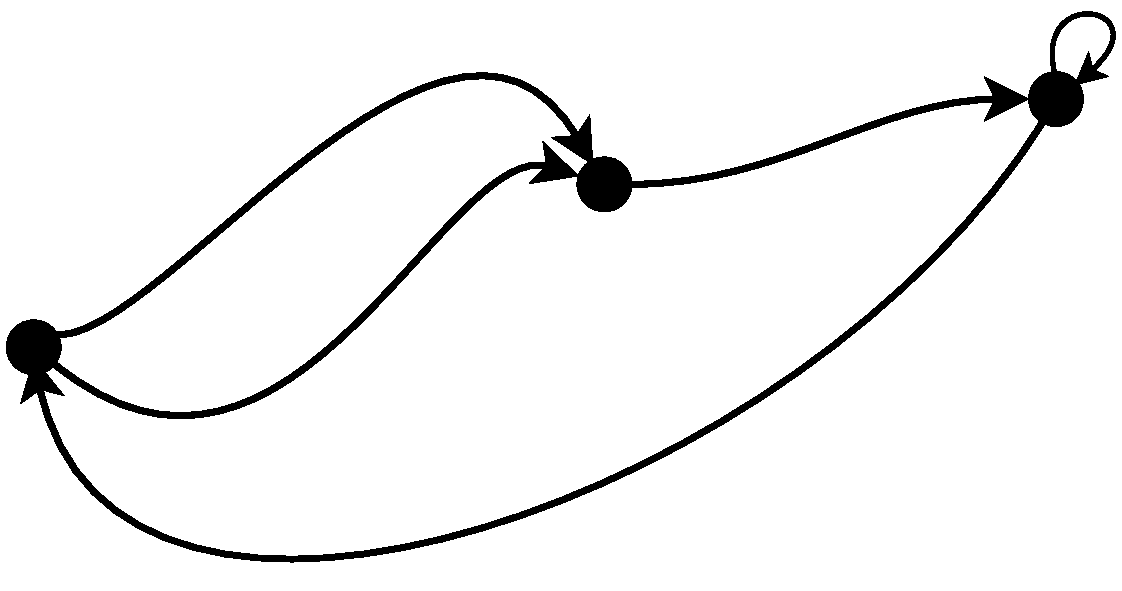
\includegraphics[scale=0.5,keepaspectratio=true]{../bilder/multigraph_bsp.pdf}
  % multigraph_bsp.pdf: 539x283 pixel, 72dpi, 19.01x9.98 cm, bb=0 0 539 283
 \end{center}
 \caption{Ein Beispiel für einen gerichteten Multigraphen: es sind sowohl Schlingen als auch mehrfache Verbindungen von zwei Knoten erlaubt}
\end{figure}

\paragraph{b)}
Sei V Menge und $E \subseteq V \times V $ ``binäre Relation auf V''
\\Dann ist $G(V,E) := (V,E, \sigma, \tau) $
\\mit $\sigma : E \rightarrow V, (p,q) \mapsto p$
\\und $\tau : E \rightarrow V, (p,q) \mapsto q$

Sei V nun z.B. die Menge $\{1,2,3\}$. Die Elemente 1,2,3 bezeichnen dabei jeweils die Knoten.
Dann ist z.B. $E = \{(1,1), (1,2), (1,3)\}$ die Menge aller Kanten des Graphen. Das heißt, es geht vom Element 1 ein Pfeil zu allen anderen Elementen und zu sich selbst.

Die Funktion $\sigma$ gibt nun zu einer Kante den Anfangspunkt als
Funktionswert zurück, also bei einer Kante $(a,b)$ das Element a):
\begin{align*}
\sigma((1,1)) = 1\\
\sigma((1,2)) = 1\\
\sigma((1,3)) = 1\\
\end{align*}
Die Funktion $\tau$ hingegen gibt jeweils den Endpunkt einer Kante
zurück, also bei einer Kante $(a,b)$ das Element b):
\begin{align*}
\tau((1,1)) = 1\\
\tau((1,2)) = 2\\
\tau((1,3)) = 3\\
\end{align*}

\begin{figure}
\centering
 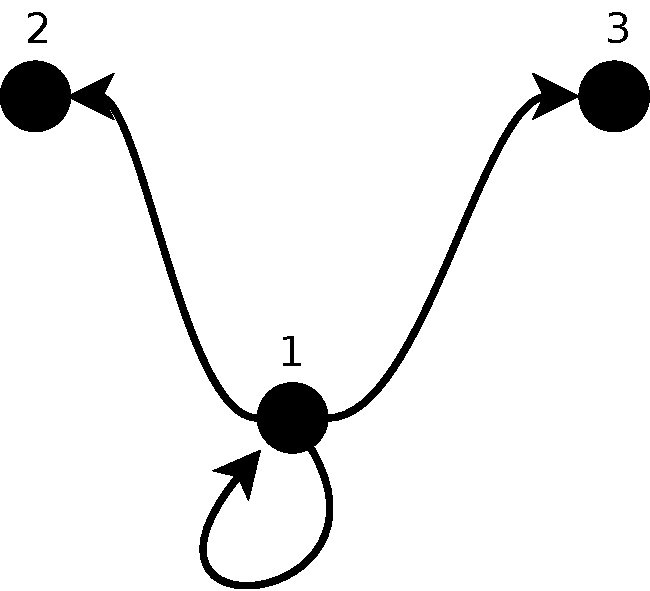
\includegraphics[scale=0.4]{./bilder/multigraph_bsp_b1.pdf}
 % multigraph_bsp_b1.pdf: 312x283 pixel, 72dpi, 11.01x9.98 cm, bb=0 0 312 283
 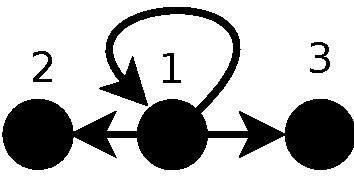
\includegraphics[scale=0.4]{./bilder/multigraph_bsp_b2.pdf}
 % multigraph_bsp_b2.pdf: 170x85 pixel, 72dpi, 6.00x3.00 cm, bb=0 0 170 85
 \caption{2 Möglichkeiten den Graphen zum Beispiel b) darzustellen}
\end{figure}

\paragraph{planarer Graph} Graph, der auf einer Ebene mit Punkten und
Linien dargestellt, keine Überscheidungen besitzt.

%%% Local Variables:
%%% mode: latex
%%% TeX-master: "../script"
%%% End:
